\documentclass[12pt]{scrartcl} %or scrbook

\usepackage{xcolor}
\definecolor{darkred}{rgb}{0.75,0,0}
\definecolor{darkblue}{rgb}{0,0,0.5}
\definecolor{darkgreen}{rgb}{0,0.5,0}
\definecolor{darkergreen}{rgb}{0,0.75,0}
\definecolor{darkmagenta}{rgb}{0.55,0,0.55}
\definecolor{left}{HTML}{041832}
\definecolor{secondary}{HTML}{241024}

\usepackage[colorlinks=true,
urlcolor=darkblue,
citecolor=darkergreen,
linkcolor=darkblue,
plainpages=false,
pdfpagelabels]{hyperref}

\setlength{\parindent}{0pt}
\setlength{\parskip}{.25cm}

\usepackage{graphicx}

\title{One Basket Finance Project}
\subtitle{Computer Science II Project}
\author{Brooke Lampe\\
\href{mailto:brooke.lampe@huskers.unl.edu}{brooke.lampe@huskers.unl.edu} \\
Department of Computer Science \& Engineering\\
University of Nebraska-Lincoln\\
}

\date{\today \\
Version 6.0
}

\begin{document}

    \maketitle
    \thispagestyle{empty}

    \vfill

    \begin{abstract}
        This document provides description and detail of the development and implementation of a new financial management system designed for One Basket Finance.  The system design utilizing the object-oriented Java programming language.
    \end{abstract}

    \newpage
    \clearpage
    \setcounter{page}{1}
    \section*{Revision History}

    \begin{tabular}{|l|l|l|l|}
        \hline
        Version & Description of Change(s) & Author(s) & Date \\
        \hline
        1.0 & Initial draft of this design document & Brooke Lampe & 2017/01/29 \\
        \hline
        2.0 & Introduction to reflect client needs, & Brooke Lampe & 2017/02/14 \\
        & further alternative design options documented, & & \\
        & description of additional functionality & & \\
        \hline
        3.0 & Database design section created & Brooke Lampe & 2017/03/01 \\
        & and additional refactoring discussed & & \\
        \hline
        4.0 & Database interface section created & Brooke Lampe & 2017/03/13 \\
        \hline
        5.0 & Sorted List ADT section created, & Brooke Lampe & 2017/03/31 \\
        & new changes and refactoring discussed, & & \\
        & and alternate design decision mentioned & & \\
        \hline
        6.0 & Added unit testing & Brooke Lampe & 2020/03/18 \\
        \hline
    \end{tabular}

    \newpage
    \tableofcontents

    \newpage
    \section{Introduction}

    The discussion of this document focuses on the project designed to replace the former financial management system of One Basket Finance.  This financial management system utilizes the object-oriented programming in the Java language.  The system manages the numerous financial services One Basket Finance provides, as well as the information of the consumers and consultants involved with the corporation.

    In an effort to preserve the efficiency and integrity of One Basket Finance's accounts, the system maintains the data pertaining to people, assets, and portfolios in distinct classes, subdividing this data into objects as needed.  The system integrates the data contained in Asset and Person objects into Portfolio objects, and provides methods for one object to access and use the information of another.  This integration includes functions capable of financial calculations related to the business activities of One Basket Finance, and it connects different aspects of the business, including people, assets, and portfolios. In addition, the system provides the availability of integration, organization, and conversion of data for usage and viewing convenience.

    Furthermore, the system provides functional ability to generate human-readable output in support of the business model of One Basket Finance.  The system is capable of aggregating information from multiple aspects of One Basket Finance and outputting this information in an organized, human-readable format.  The system is designed to be accessible and understandable by One Basket Finance and strives to present data in a manner that is greatly enhanced from the original flat files.

    \subsection{Purpose of this Document}

    The purpose of this document is to detail the structure and diversified application of this financial management system.  It discusses the utilization of object-oriented programming to represent both abstract and concrete entities as digital objects.  This document provides the client with information pertinent to running and maintaining the system.  The document should provide sufficient detail for the client to build additional functionality into this system if needed.

    \subsection{Scope of the Project}

    This financial management system will be used to process, store, and organize the data pertaining to One Basket Finance.  This system will also allow the data to be integrated and organized for viewing convenience.  This system will replace One Basket Finance's current AS400 green-screen system, which is out of date.  This system will support OBF's business model, abide by OBF's rules and regulations, and provide important functional support.  Functions include the management of various assets as well as assessment of the investment through several business calculations, including risk and return.  The system will also provide functional capabilities to record and maintain broker information.  Further, the system utilizes a database in order to maintain secure and normalized data.  The Java aspect of the system abides by the best practices of object-oriented programming; similarly, the database aspect complies with relational database management system requirements and best practices.

    \subsection{Definitions, Acronyms, Abbreviations}

    \subsubsection{Definitions}

    Abstract class - A class that cannot be directly constructed, one that can be constructed only through construction of some of its subclasses.[2].

    Abstraction - The ability to provide usable objects and methods but without providing details of how they work.

    Class - A set of objects having the same behavior (but typically differing in state), or a template defining such a set.[2]

    Constructor - A class method (in object-oriented programming) that creates and initializes each instance of an object.[2]

    Encapsulation - The ability to group and protect data and the methods that act on the data.

    Exception - An interruption in normal processing, especially as caused by an error condition.[2]

    Functional Programming - Programming style in which data and functions tend toward having more in common with each other while offering more flexibility in terms of how functions are actually used.  Algorithms tend also to be defined in terms of recursion and composition rather than loops and iteration.[3]

    Inheritance - The ability to easily construct new data types or classes by extending existing structures, data types, or classes.[1]

    Java - Object oriented language that has a C-like syntax.[1]

    Mutator - A method that is permitted to change the state of the object to which it is applied.[1]

    MySQL - Open source relational database management system owned by Oracle Corporation.

    Object - An instance of a class.[2]

    Object-Oriented Programming - Using entities called objects that can process data and exchange messages with other objects.[2]

    Polymorphism - The ability of a function to apply to more than one type of object or data.[1]

    Subclass - In object-oriented programming, an object class derived from another class (its superclass) from which it inherits a base set of properties and methods.[2]

    Procedural Programming - Programming style in which data tends to be highly decoupled from the functions that operate on it.[3]

    Superclass - A class that passes attributes and methods down the hierarchy to subclasses.[2]

    \subsubsection{Abbreviations \& Acronyms}

    ACID - Atomicity, Consistency, Isolation, Durability - set of properties of database transactions

    ADT - Abstract Data Type

    API - Application Programming Interface

    CRUD - Create, Retrieve, Update, and Destroy - the four main functions of persistent storage

    DDL - Document Data Language

    JDBC - Java Database Connectivity

    JPA - Java Persistence API

    JSON - JavaScript Object Notation

    OBF - One Basket Finance

    OOP - Object-Oriented Programming

    RDBMS - Relation Database Management System

    SQL - Structured Query Language

    XML - Extensible Markup Language

    \section{Overall Design Description}

    This system was developed to represent assets, people, and portfolios, with such entities modeled in the form of objects in the Java OOP paradigm.  The relationships between these objects will be the foundation of OBF's financial management system.

    The two primary objects modeled by the system are assets and people, although the system also represents secondary objects, such as addresses, as objects.  The four main principles of OOP:  abstraction, encapsulation, inheritance, and polymorphism, have been implemented in the design of the system and applied to assets and people modeled by the system.

    Abstraction is applied by creating distinct classes with distinct methods that are accessible by other classes.  The class accessing the method does not need or have access to the details of the method, it merely offers an input and receives an output.

    Encapsulation comes in the form of several distinct classes, capable of functioning independently, that are used to input, store, and output data.  Each class strives to organize and protect its data.  The variables in the class are generally given private status and only accessible by getters; thus, they are immutable.  The exception occurs when parsing data pertaining to portfolios.  The Portfolio object contains a list of assets associated with the portfolio, including how much of that asset is owned by the portfolio, i.e. the balance of a deposit account, the percent stake of a private investment, or the amount of shares in a stock asset.  This information is specific to the portfolio, so copies of the assets are created and this information is provided to the asset through a setter method.  The original asset is not compromised; however, because the setter method is called on copies of the asset.

    Though there are three distinct assets (deposit accounts, private investments, and stocks) modeled by the system, they share a number of commonalities and are stored in the same list of assets.  As such, it is important that some methods can interact with assets without knowing which type of asset they are.  This is achieved through inheritance.  The Asset class contains several general methods that are overridden by its subclasses.  These methods can be called without knowing the specific asset type, and include several getters as well as methods pertaining to risk, annual return, and total value of the asset.

    Polymorphism is closely tied to inheritance in this system as DepositAccounts objects, PrivateInvestment objects, and Stocks objects are referred to by the superclass, Asset, in order to store them all in an Asset list.  Polymorphism also dispels concerns about knowing the type of the object in order to use a method on it.  Several processes share the same method name, but the method pertaining to the specific asset is the one that is applied.

    \subsection{Alternative Design Options}

    An alterative design structure could have involved an approach other than OOP, such as procedural programming or functional programming.  Procedural programming would have involved a step by step process centered around the main in which the data is manipulated by a function at each step.  The procedural programming paradigm would not have fit well with the problem and functional requirements presented, as the entities modeled by the system belong in particular groups more so than a particular order.  A second option could have been functional programming, which involves composition and recursion.  Composition has been used in the development of this system, but recursion is typically not a best practice, so function programming style was not used.

    An alternative design option would have involved limited utilization of the inheritance feature of objects.  As it is now, the Asset class is extended by each of the three types of objects such that common methods can be reused conveniently, yet methods specific to different types of assets within the Asset class are maintained separately.  An alternative to inheritance would be composition; that is, one class maintaining a reference to an instance of another class.  Preference for composition stems from the potential for methods of extended classes to be overridden such that they have inappropriate or inconsistent behavior.  For this system; however, the reused methods maintain a consistent purpose.  An additional concern with inheritance is setter methods that would allow violation of the semantics of an object.  This issue is avoided by avoiding the use of setters.

    When developing the sorted list ADT, an alternate design option was to use an array-based list.  An array-based list can be parameterized similarly to the linked list that was used; however, it cannot be instantiated generically.  Users would be forced to use a raw type and cast, which, although feasible, is not ideal.  Furthermore, resizing an array-based list would require new memory allocation, all the elements of the array-based list would have to be copied, and there is potential for wasted memory.  A linked list can be more conveniently parameterized and does not require a fixed size nor resizing.  For that reason, the array-based list design was foregone in favor of a linked list ADT.

    \section{Detailed Component Description}

    The following sections provide detail of the various components of the system, including the Java classes, objects, and methods used to appropriately represent the data.

    \subsection{Database Design}

    The database design reflects the structure of the classes implemented in the Java program.  The relationships between tables in the database are similar to the relationships between classes in the Java program.  In addition, the tables respect the conventions of one-to-many and many-to-many relationships.  The person table contains records for all the people held in the database.  The person table has an integer primary key that is used only by the database, is not allowed to be null, and is auto-incremented, called personId.  The person table contains the personCode that identified an individual in the old financial management system; the personCode cannot be null and has a constraint that requires it to be unique.  In addition, the person table contains records for first name, last name, and the individual's address separated into its components.  The individual's last name must not be null, the remaining data is allowed to be null.  The person table also contains fields for broker classification and broker identification.  These fields are null unless the person is a broker.  The broker identification has a constraint that requires it to be unique.

    The email table contains the email addresses of all the individuals in the person table, seeing as one individual can have multiple email addresses.  The email table has an integer primary key controlled and auto-incremented by the database and not allowed to be null, called emailId.  The email table uses the primary key of the person table as a foreign key in order to connect an individual to his or her emails.  The emailAddress field of the email table is not allowed to be null, as there is no point in listing a personId and an emailId without an email address.

    The portfolio table contains the portfolioCode that identified the portfolio in the old system, as well as the names of the owner, manager, and optional beneficiary.  The list of assets is not included in the portfolio table because one portfolio may own many assets, and one asset may be owned by many portfolios.  The table has an integer primary key not allowed to be null that is controlled and auto-incremented by the database.  The table also contains foreign keys that reference an individual in the person table, called ownerId, managerId, and beneficiaryId.  All of these fields are allowed to be null.  This decision was made because during a change of ownership or manager, or if the beneficiary inherits the portfolio, the portfolio should not be deleted from the system.  If One Basket Finance has not sold a portfolio to an owner, then the field should remain null until an owner is found, rather than deleting from the system.  The same is true if a manager leaves the firm and a new manager has not been found for the portfolio.  The beneficiary field is optional, so it also allowed to be null.  Because the same person could own, manage, or be the beneficiary of multiple portfolios, these fields are not required to be unique.  As it is now, the system does not allow multiple people to own the same portfolio, but it does allow the same person to own multiple portfolios, so the database models a one-to-many relationship between the person table and the portfolio table.

    The asset table stores all of the assets owned by all of the portfolios available to One Basket Finance.  The information contained in this table is not specific to particular people or portfolios; rather, it is general information about the asset that is true regardless of ownership.  Therefore, this table does not reference the person table or the portfolio table.  It has an auto-incremented, not null, integer primary key.  In addition, it holds the assetCode used by the old system to uniquely identify an asset; this field is not allowed to be null and is required to be unique.  Assets include deposit accounts, stocks, and private investments, each of which have different related information.  All possible fields for an asset are stored in the same asset table, and if a field is not applicable to a particular asset, it is left null.  This structure favors best practices of databases, as designing different tables for each asset would require several one-to-one relationships with the asset table, and one-to-one relationships are generally a poor design.  Furthermore, this arrangement will allow greater compatibility when used with the Java system, as all of the assets are stored in the same place and can be treated the same.

    The fifth and final table is the equity table, which is a join table for the portfolio table and the asset table.  The portfolio table and the asset table have a many-to-many relationship; thus, the join table was needed.  The equity table has its own auto-incremented, not null primary key, as well as foreign keys to connect to the portfolio table and the asset table, portfolioId and assetId, respectively.  These fields cannot be null; otherwise, the equity table would be unable to join the values of the other two tables.  The equity table also includes a field called worth, which has a different meaning depending upon the asset.  For a deposit account, worth refers to balance; for a stock, worth refers to number of shares; for a private investment, worth refers to percent stake.  These fields are specific to the portfolio and to the asset, which is the reason they are stored in the join table.

    For further illustration, refer to \textbf{Figure 1}.

    \graphicspath{{Z:/Design Document/}}
    \begin{figure}[!ht]
        \centering
        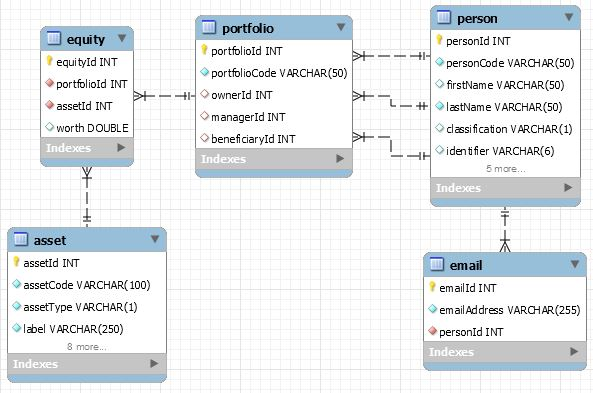
\includegraphics[scale=1]{portfolioModel.jpg}
        \caption{An illustration of the relationships between tables in PortfolioDB}
        \label{Figure 1:  Database Tables}
    \end{figure}

    \subsubsection{Component Testing Strategy}

    The database portfolioDB.sql was tested through queries conducted on test data.  Test queries are stored in portfolioQueries.sql and will also be implemented in the system.  The queries tested all four aspects of CRUD.  The queries included inserting data into the person table, the email table, the portfolio table, the asset table, and the equity table, fulfilling the create aspect of CRUD.  The queries also retrieved specific data and included joining two or more tables together in order to aggregate information from multiple tables.  This fulfills the retrieve aspect of CRUD.  An email address was updated in order to fulfill the update aspect of CRUD.  To fulfill the destroy aspect of CRUD, a record was deleted from the person table.  To achieve this, records that referenced the person had to be deleted first from child tables.  The email addresses of the person were deleted from the email table, and the portfolio records referencing the person were updated to null.  The portfolio records were changed to null rather than deleted because several of the portfolios were owned by different people, and in the business application, the portfolios would not be deleted if the manager was changed.  The portfolios owned by the person were also changed to null instead of deleted, as those portfolios were still managed by One Basket Finance.  Once all the records pertaining to the person were deleted, the person was also deleted.  This was confirmed through queries that showed all records in all the tables.  An additional query was performed to insert the deleted person into the person table as well as an email address in the email table.  The query was successful and did not violate uniqueness constraints on the personCode, which shows the the person had been successfully deleted before being inserted again.

    \subsection{Class/Entity Model}

    As mentioned above, the two primary objects represented by this system are assets and people, contained in the Asset and Person classes, respectively.  The remaining classes stem from or act upon or relate to these two classes.  The Person class contains instances of the Broker object, the Name object, and the Address object.  The Broker object two pertinent pieces of information with regard to a person who is also a broker.  The Name object contains the first name and last name of each person.  The choice to maintain the first name and last name in a separate object was made in order to support potential future functionality, such as sort or filter methods that seek a specific first name or last name.  The Address object is given its own class because addresses are relevant to business and organization data as well as person data.  The Portfolio class maintains the overall portfolio, and contains Person objects and Asset objects.  It is an example of a class that is largely built from the two primary objects.  It provides functionality to connect people to the assets they own and provides numerical information about the assets.

    Another important class is the Parse class, which contains a method to parse a line containing person information into a Person object or an Asset object, as well as a method to parse a line containing portfolio information, call a search method, and connect Person and Asset objects to the portfolio in order to create a Portfolio object.  The Search class contains methods to search for an Asset object or a Person object given an assetCode or a personCode, respectively.  All three Parse methods are called by the Driver class, which contains the main execution code for the project.  The Driver class also calls the getFileLines method from the GetFileLines object, which reads a file line by line and stores each line in an array.  The Driver class is also responsible for calling methods that export to .xml and .json file formats, as well as calling a method from the Summary class to organize, summarize, and output portfolio information to the standard output.

    For further illustration, refer to \textbf{Figure 2}.

    \graphicspath{{Z:/Design Document/}}
    \begin{figure}[!ht]
        \centering
        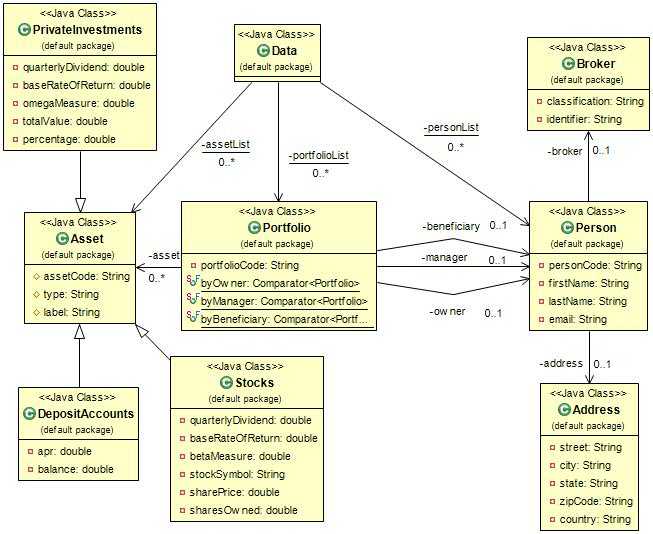
\includegraphics[scale=0.7]{entities.jpg}
        \caption{An illustration of the relationships between Asset, Person, and Portfolio classes}
        \label{Figure 2:  Classes and Entities}
    \end{figure}

    \subsubsection{Component Testing Strategy}

    The testing of the classes and objects involved in this program was done primarily through file input and output.  A plain text file containing lines of data was read in by the program.  The program parsed and stored this data, and then exported the output as .xml and .json files.  By comparing the data from the plain text file to the data contained in the .xml and .json files, testers could confirm that the correct data was read in, stored, and exported.  The .xml and .json files were also validated by an online tool to confirm that they were properly structured and formatted.  A sample file input and an expected file output in both .xml and .json file formats for both the assets data and the persons data was created in order to test the files.  In addition, the Portfolio class was tested through sample input that was compared to an expected output stored in a .txt file.  The summary generated and sent to the standard output by the Summary class and the Portfolio class had to match the expected output.  This process was done with both the professor's test cases and a test case generated by the student.  In addition, black box testing was performed by an online testing system, webgrader.

    \subsection{Database Interface}

    The API for the financial management system follows the best practices of abstraction, encapsulation, inheritance, and polymorphism.  The connection to the database is handled by the Connect class, which contains a method to connect to the database and a method to disconnect from the database.  Both of these factory methods are used for all connections to the database.  All connections are properly disconnected when no longer needed in order to avoid the loss of resources.  Responsibility for a connection is maintained by the method that called for the connection; that is, the method that opened the connection closes the connection.  The connection is not passed to other methods, as this would violate the single-responsibility principle.  If a method calls a connection and then calls another method that needs a connection, the called method will create and close its own connection.

    Three classes are responsible for loading the data from the database:  LoadAsset, LoadPerson, and LoadPortfolio.  The LoadAsset class is responsible for loading the asset entries from the asset table of the database into Asset objects.  The LoadPerson class is responsible for loading data pertaining to Person objects from the database into Person objects.  This class is required to obtain data from multiple tables, including the person table, the state table, the country table, and the email table.  Each SQL statement is separated out into its own method and grouped appropriately, in keeping with good abstraction and encapsulation practices.  The method that loads information from the database into Person objects is contained in the LoadPerson class.  The method that searches the database for a state matching a stateId, as well as the method that searches the database for a country matching a countryId, is stored in the Search class.  Another method searches for all the email addresses associated with a specific personId and organizes them into a comma-delimited list, which is returned by the function.  The email field of a Person object is a string, so the emails have to be stored as a string.  Further, the comma-delimited email list maintains compatibility with the methods that convert Person objects to JSON or XML file formats.

    The Log class contains a logger instance and its configuration.  This class is used to log errors, such as SQLExceptions, for viewing convenience later on.  This class was implemented in order to abide by the best practice of configuring errors to be logged in the most appropriate location.  The Log class uses log4j, through a jar file stored on the build path.

    The PortfolioData class contains methods to manipulate the database, portfolioDB.  It is capable of adding, updating, and removing entries from various tables in the database.  Certain elements are used frequently, such as features to search for personId, assetId, and portfolioId; therefore, these elements are contained in the Search class as helper methods to the methods that add, update, and remove from the database.  Maintaining these methods in the Search class follows the principles of abstraction and encapsulation, and provides greater reusability of the methods.  All classes and methods that interact with the database do so using Prepared Statements.  Prepared Statements sanitize input, protecting the database from SQL Injection Attack.

    \subsubsection{Component Testing Strategy}

    The functionality of the API responsible for loading of information from the database was extensively tested by manipulating the entries in the database and then running the API to ensure that it functioned appropriately.  In the database, entries were added to various tables with null values for all fields allowed to be null, and the database was tested to ensure that it was still able to produce a summary report and the null values were appropriately handled.  The database was given unusual entries in order to probe and break potentially weak code.  The code was also uploaded to the webhandin and tested on the webgrader to ensure that it ran correctly on the cse server.

    The functionality of the API responsible for manipulating the information in the database was tested by changing the information through the database and changing the information through the use of the API and comparing the results.  Corner cases were tested extensively in the Eclipse environment by providing null input data in all fields allowed to be null.  In addition, the program was tested by inserting empty strings.  This component was also tested through the webgrader, which removed the original data entries using the methods of the Add class and the Remove class and also tested additional test cases.

    \subsection{Design \& Integration of Data Structures}

    The sorted list ADT used by the system is located in the SortedList class, and an instance of a SortedList can be created using a constructor.  A sorted list instance is generic, so the constructor expects a parameter to be given, and a warning will result if the constructor is not parameterized.  In addition, the constructor requires two arguments, a head element, which would initially be null, and a comparator to compare the elements of the list in order to maintain sorted order.

    The SortedList class is implemented using linked list structure.  The list references the head element, the head element references the next element, and this pattern continues through the list, with each element in the list holding the reference to the next element.  The linked list structure does not have a fixed size; therefore, there is no resizing in response to the addition or removal of an element.  Thus, the capacity of the list does not expand or contract.  The number of elements in the list; however, can be determined by iterating through the linked list until the current element points to null.  Operations on the list involve changes in references, not the elements.

    Order is maintained in the sorted list ADT by inserting a new element in the position that is in keeping with the order of the list.  When a user calls the insert method, the method first uses the given comparator to compare the new element to existing elements in the list in order to determine the correct index at which to insert the new element.  The correct index value follows smaller elements and precedes larger elements.  In the event that two elements are equal, the decision was made in the design to place the new element following the original element.  Of course, if the two elements are the same, then the position of each element with respect to the other is interchangeable.  Once the proper index for the new element is determined, the appropriate method is called.  There are three methods that can be called by the insert method to insert the new element.  They are insertElementAtStart, insertElementAtIndex, and insertElementAtEnd.  They are private methods inaccessible to the main of the program; rather, they are used solely by the SortedList class.  The private status of the three methods ensures that order is maintained in the sorted list ADT.  If the three methods were accessible to the main of the program, then a user would be able to insert an element into the list wherever he or she wanted, without regard to order.

    Furthermore, the three separate methods are important because they handle corner cases.  A different process is required to insert an element at the start or end of the list than to insert in the middle, particularly if the element to be inserted is the first element in a new, empty list.  To add an element to the beginning of the list, the head node must be set to the new node pertaining to the new element.  To add an element to the end of the list, the setNext method of the Node class must be called in order to set the final node pointing to the new element.  To insert an element at an index value that is not one of the corner cases, the node at the previous index is told to point to the new element, and the node of the new element is told to point to the element that was previously in its position.  If insertElementAtIndex is called with one of the corner cases, then the method pertaining to that corner case is called.  This process facilitates code reuse.  In addition, there is a method for batch insertion in the form of an ArrayList that iterates over the ArrayList and calls a method to insert each element.

    When removing an element or elements, there is no impact on the order of the list, so there are multiple methods the user can call to remove an element or elements.  In addition, there are fewer corner cases with regard to removing elements, so these cases are all handled within the method instead of calling another method to handle it.  The removeElementAtIndex removes an element at a specific index from the list.  If the element is the head element, then the head element is set to the next element in the list.  If the element is elsewhere in the list, the reference preceding it is told to point to the reference succeeding it, removing the element.  There is no corner case at the end of the list because if the last element is to be removed, the preceding element will be forced to point to the element after the last element, which is null.  The preceding element then becomes the last element.  There is also a method to remove the first instance of an element, and it does so by comparing the elements and then eliminating the first match.  Moreover, there is a removeAll method that removes all elements merely by setting the head element to null.

    To retrieve an element, there is a get method that calls a getNode method.  The getNode method iterates through the list until it reaches the node at the given index.  This node is then returned.  The get method receives the node that was returned and the getElement method from the Node class is called in order to retrieve the element associated with the node.

    The implementation of an instance of the SortedList class is generic and can hold Portfolio objects or other types of objects.  This is the principle of parameterized polymorphism.

    \subsubsection{Component Testing Strategy}

    This component was tested extensively by using all of the methods associated with the SortedList class.  An instance of the SortedList class was used to hold the Portfolio objects that had been loaded from the database into an ArrayList.  The batch version of the insert method was used to insert the entire ArrayList into an instance of the SortedList.  A summary report and a detail report were then printed.

    This process was completed with four different comparators.  The first comparator was by owner name, the second was by total value of the portfolio from least to greatest, the third was total value of the portfolio from greatest to least, and the fourth was broker type followed by broker name.  The results of these tests were then compared to the results when using the original ArrayList in conjunction with Collections.sort and a comparator.  Apart from one exception thrown due to a typo in the code, there were no other issues.  The tests showed accurate, reliable results.

    To confirm the accuracy and consistency of SortedList instances, the data in the database was updated to include more brokers.  In the original test cases, the reliability of the fourth comparator, which compared using broker type and then broker name, could not be confirmed because all of the expert brokers had names earlier in the alphabet and all of the junior brokers had names later in the alphabet.  The new brokers had names and classifications that would reveal whether or not the fourth comparator was working properly.  When the new test cases were used, all of the test cases were correct.

    The other aspects of the sorted list ADT, such as the regular insert method, the retrieve method, and the various remove methods, were also tested by adding, retrieving, and removing random elements from the original ArrayList.  These tests cases also showed accurate outcomes.

    The SortedList class was then tested through the webgrader with various test cases designed to break bad code, and again, the results were accurate and consistent.

    \subsection{Changes \& Refactoring}

    Previously, the data parsed by the system was stored in Asset objects and Person objects in an array in the main method of the main driver class.  The array structure was refactored in favor of a dynamic data container, the ArrayList.  The ArrayList does not require a specified size and is more convenient for adding or removing objects.  Adding to an array would require creating a larger array and copying over the data, removing from an array would require creating a smaller array and copying over the data.  The ArrayList is automatically resized for data changes and provides greater usability.  In addition, the system data is now stored in the Data class, where it is maintained and accessible by other classes through getter methods.  This refactoring stores the data in a more secure location where it is immutable and cannot be directly manipulated by the driver class.  In addition, storing the data outside of the main method allows it to be accessible to methods in other classes without having to pass the data to all the methods that need it.

    The initial structure of classes included a Name class intended to faciliate searching and sorting by first name, last name, and additional names if applicable.  The Name class appears to be an example of excessive abstraction, so it has been removed in favor of a firstName string and lastName string in the Person class.  Searching and sorting will enlist the use of the two strings instead of an additional class.

    The names of the classes containing assets, persons, and portfolios were originally Assets, Persons, and Portfolios.  The classes and all uses of the classes have been renamed Asset, Person, and Portfolio, respectively.  This refactoring was done to align with the naming conventions of the database, PortfolioDB.  It is best practice with a database to use singular nouns to name the tables because it is difficult to remember whether or not the plural form was used.  To use singular tables in the database and plural classes in the Java system would be inconsistent and difficult to remember.  Thus, the Java classes were renamed to align with the singular noun best practice used when creating the database.

    Ultimately, the system was refactored such that information is loaded directly from the database instead of loading from flat files.  As a result, several new classes were created to load each of the main object types, Asset objects, Person objects, and Portfolio objects.  The driver class restructured to call on methods from the LoadAsset, LoadPerson, and LoadPortfolio classes instead of the Parse class, which is no longer in use.

    With the development of a sorted list ADT to store Portfolio objects in place of the ArrayList previously used, the Summary class was refactored to obtain data from the sorted list ADT rather than the ArrayList.  Several of the methods in the Summary class involve the summation of information from all the portfolios.  These methods previously required no argument and called the PortfolioList from the Data class to obtain the information needed.  The Summary class had to be adjusted so that the summation methods obtained information from the sorted list ADT.  To preserve the usability of the previous methods, the system utilizes the principle of polymorphism.  If the method is called without an argument, the original ArrayList is used to provide the portfolio information.  If the method is called with a sorted list as an argument, then the new sorted list ADT is used to provide the portfolio information.

    In addition, the Summary class contained a method called printSummary, which would print a summary and detail report for the portfolios.  This method was split into two methods, printSummary and printDetailReport, which print a summary report and a detail report, respectively.

    \subsection{Unit Testing}

    This project leverages JUnit for its unit testing framework, which seeks to validate that the method under test performs as expected in all cases, including corner cases. Furthermore, this unit testing behavior helps to catch errors arising from updating and refactoring the project. In effect, the unit tests serve as regression tests.

    The unit testing of this project is strictly proof of concept, as this project is not intended for production use. Should the project be adopted as a live solution with real users, then additional unit testing would prove necessary. The proof of concept unit testing functionality exists for the Search class, and the unit tests corresponding to this class live in the SearchTest class class in the com.sdb.test package.

    \section{Additional Material}

    This section provides additional material useful to the client and others interested in the design of the system, including a bibliography for further reading.

    \subsection{Bibliography}

    [1]California State University, San Bernardino. (2011, May 31). Glossary of Computer Programming Terms. Retrieved February 01, 2017, from \url{<http://cse.csusb.edu/dick/cs202/glossary.html>}

    [2]Wiktionary. (2016, April 20). Glossary of Computer Programming. Retrieved February 01, 2017, from \url{<https://en.wiktionary.org/wiki/Appendix:Glossary_of_computer_programming>}

    [3]Stack Overflow.  (2009, Feb 16).  OOP vs Functional Programming vs Procedural Programming.  Retrieved February 11, 2017, from
    \url{<http://stackoverflow.com/questions/552336/oop-vs-functional-programming-vs-procedural>}

\end{document} 